% !TEX TS-program = latexmk

\documentclass[12pt,twoside]{book}

% Verificacion de sintaxis sin producir salida:
% descomentar la segunda linea para verificar
% sintaxis sin producir salida.
\usepackage{syntonly}
% \syntaxonly

% Palabras clave en distintos idiomas
%\usepackage[activeacute]{babel}

% Patrones para division en silabas
\hyphenation{par-ti-cu-lar}

% Inclusion de imagenes
\usepackage{graphicx}

% Codificacion de simbolos
\usepackage[T1]{fontenc}
\usepackage[applemac]{inputenc}

% Fuentes y simbolos adicionales
\usepackage{amsfonts}
\usepackage{amsmath}
\usepackage{amssymb}
\usepackage{mathrsfs}

% Bullets especiales
\usepackage{enumerate}

% Colores
\usepackage[table]{xcolor}

%TODO
\usepackage{todonotes}

\definecolor{verdeOscuro}{rgb}{0,0.6,0}
\definecolor{verdeAzulado}{RGB}{3,168,108}
\definecolor{gris}{rgb}{0.5,0.5,0.5}
\definecolor{malva}{rgb}{0.58,0,0.82}
\definecolor{grisClaro}{rgb}{0.92,0.92,0.92}

% Vinculos
\usepackage{hyperref}
\hypersetup{
  colorlinks,
  urlcolor={malva}
}

% Algoritmos
\usepackage[ruled,lined,linesnumbered,commentsnumbered]{algorithm2e}

%\usepackage[all]{xy}

% Generacion de dibujos con TeX
\usepackage{tikz}
\usetikzlibrary{arrows,shapes,matrix,decorations,calc,positioning}
\tikzstyle{arc}   =[->,shorten <=3pt, shorten >=3pt,
                   >=stealth, line width=1.1pt]
\tikzstyle{edge}  =[shorten <=2pt, shorten >=2pt,
                    >=stealth, line width=1.1pt]
\tikzstyle{myloop}=[style={},shorten <=1pt, shorten >=1pt,
                    >=stealth, line width=1.1pt, loop]
\tikzstyle{vertex}=[circle, draw, minimum size=6pt,
                    line width=0.75pt, inner sep=0pt,
                    outer sep=0pt]
\tikzstyle{label} =[inner sep=1pt, fill=none, draw=none]


% Ajuste de parametros en la pagina
\usepackage{geometry}

% Ubicacion precisa de floats
\usepackage{float}

% Manejo de encabezados
\usepackage{fancyhdr}

% Estilo de encabezados
\pagestyle{fancy}
\renewcommand{\chaptermark}[1]{\markboth{#1}{}}
\renewcommand{\sectionmark}[1]{\markright{\thesection\ #1}}
\fancyhf{}
\fancyhead[LE,RO]{\textsc{\bfseries\nouppercase\thepage}}
\fancyhead[LO]{\textsc{\bfseries\nouppercase\rightmark}}
\fancyhead[RE]{\textsc{\bfseries\nouppercase\leftmark}}
\renewcommand{\headrulewidth}{0.5pt}
\renewcommand{\footrulewidth}{0pt}
\addtolength{\headheight}{3pt}
\fancypagestyle{plain}{
  \fancyhead{}
  \renewcommand{\headrulewidth}{0pt}
}

% Delimitadores para terminar las demostraciones
\newcommand{\blackqed}{\hfill$\blacksquare$}
\newcommand{\whiteqed}{\hfill$\square$}
\newcounter{proofcount}

% Generacion de tabla de contenidos
\usepackage{makeidx}
\makeindex

% Ambientes de teorema y demostracion
\usepackage{amsthm}

% Referencias con nombres automaticos
\usepackage{cleveref}

% Definiciones de nuevos ambientes
\newtheorem{theorem}{Theorem}[section]
\newtheorem{lemma}[theorem]{Lemma}
\newtheorem{proposition}[theorem]{Proposition}
\newtheorem{corollary}[theorem]{Corollary}

\theoremstyle{definition}
\newtheorem{definition}[theorem]{Definition}

% Redefinicion para que las demostraciones terminen con cuadrito negro
\renewenvironment{proof}[1][\proofname.]{\par
\ifnum \theproofcount>0 \pushQED{\whiteqed} \else \pushQED{\blackqed} \fi%
\refstepcounter{proofcount}
%
\normalfont %\topsep6\p@\@plus6\p@\relax
\trivlist
\item[\hskip\labelsep
\itshape
\textbf{\textit{#1}}]\ignorespaces
}{%
\addtocounter{proofcount}{-1}
\popQED\endtrivlist
}

% Macros
% Abreviatura para fuentes true type
\newcommand{\ttt}[1]{%
\texttt{#1}%
}

\newcommand{\indice}[1]{%
\textbf{#1}\index{#1}%
}

\newcommand{\indiceSub}[2]{%
\textbf{#2}\index{#1!#2}%
}

%Macros para delimitadores
\renewcommand{\l}[1]{\left\{#1\right\}}
\newcommand{\p}[1]{\left(#1\right)}

\begin{document}

\frontmatter

\include{caratula}
\include{hojadedatos}
\chapter*{Acknowledgements}
\addcontentsline{toc}{chapter}{Acknowledgements}

Agradezco a mi director de tesis por haber hecho esta plantilla.

\tableofcontents


\mainmatter

\chapter{Introduction}
\label{cha:intro}

%%%%%%%%%%%%%%%%%%%%%%%%%%%%%%%%%%%%%%%%%%%%%%%%%%%%%%%%%%%%%%%%%%%%%%%%%%%%%%%%
%%%%%%%%%%%%%%%%%%%%%%%%%%%%%%%%%%%%%%%%%%%%%%%%%%%%%%%%%%%%%%%%%%%%%%%%%%%%%%%%
%%%%%%%%%%%%%%%%%%%%%%%%%%%%%%%%%%%%%%%%%%%%%%%%%%%%%%%%%%%%%%%%%%%%%%%%%%%%%%%%
%%%%%%%%%%%%%%%%%%%%%%%%%%%%%%%%%%%%%%%%%%%%%%%%%%%%%%%%%%%%%%%%%%%%%%%%%%%%%%%%
\section{Graphs}
\label{sec:graphs}

%TODO: Definiciones no estándar.


%%%%%%%%%%%%%%%%%%%%%%%%%%%%%%%%%%%%%%%%%%%%%%%%%%%%%%%%%%%%%%%%%%%%%%%%%%%%%%%%
%%%%%%%%%%%%%%%%%%%%%%%%%%%%%%%%%%%%%%%%%%%%%%%%%%%%%%%%%%%%%%%%%%%%%%%%%%%%%%%%
%%%%%%%%%%%%%%%%%%%%%%%%%%%%%%%%%%%%%%%%%%%%%%%%%%%%%%%%%%%%%%%%%%%%%%%%%%%%%%%%
%%%%%%%%%%%%%%%%%%%%%%%%%%%%%%%%%%%%%%%%%%%%%%%%%%%%%%%%%%%%%%%%%%%%%%%%%%%%%%%%
\section{Hereditary properties}
\label{sec:hereditary}

%TODO: Obstrucciones, libres de F, consecuencias basicas de la definicion.


%%%%%%%%%%%%%%%%%%%%%%%%%%%%%%%%%%%%%%%%%%%%%%%%%%%%%%%%%%%%%%%%%%%%%%%%%%%%%%%%
%%%%%%%%%%%%%%%%%%%%%%%%%%%%%%%%%%%%%%%%%%%%%%%%%%%%%%%%%%%%%%%%%%%%%%%%%%%%%%%%
%%%%%%%%%%%%%%%%%%%%%%%%%%%%%%%%%%%%%%%%%%%%%%%%%%%%%%%%%%%%%%%%%%%%%%%%%%%%%%%%
%%%%%%%%%%%%%%%%%%%%%%%%%%%%%%%%%%%%%%%%%%%%%%%%%%%%%%%%%%%%%%%%%%%%%%%%%%%%%%%%
\section{Chordal graphs and its subclasses}
\label{sec:chordal-defs}

%TODO: Definicion cordal, caracterizaciones relevantes (peo), linealidad de clan maximo y similares.

%TODO: Definicion split y caracterizaciones relevantes. Reconocimiento en tiempo lineal (sucesion de grados y algoritmo certificador).



%%%%%%%%%%%%%%%%%%%%%%%%%%%%%%%%%%%%%%%%%%%%%%%%%%%%%%%%%%%%%%%%%%%%%%%%%%%%%%%%
%%%%%%%%%%%%%%%%%%%%%%%%%%%%%%%%%%%%%%%%%%%%%%%%%%%%%%%%%%%%%%%%%%%%%%%%%%%%%%%%
%%%%%%%%%%%%%%%%%%%%%%%%%%%%%%%%%%%%%%%%%%%%%%%%%%%%%%%%%%%%%%%%%%%%%%%%%%%%%%%%
%%%%%%%%%%%%%%%%%%%%%%%%%%%%%%%%%%%%%%%%%%%%%%%%%%%%%%%%%%%%%%%%%%%%%%%%%%%%%%%%
\section{Exact neighbourhoods}
\label{sec:exact-neigh}

%TODO: Definiciones de vecindades exactas y breve explicacion de como calcularlas en tiempo lineal.



%%%%%%%%%%%%%%%%%%%%%%%%%%%%%%%%%%%%%%%%%%%%%%%%%%%%%%%%%%%%%%%%%%%%%%%%%%%%%%%%
%%%%%%%%%%%%%%%%%%%%%%%%%%%%%%%%%%%%%%%%%%%%%%%%%%%%%%%%%%%%%%%%%%%%%%%%%%%%%%%%
%%%%%%%%%%%%%%%%%%%%%%%%%%%%%%%%%%%%%%%%%%%%%%%%%%%%%%%%%%%%%%%%%%%%%%%%%%%%%%%%
%%%%%%%%%%%%%%%%%%%%%%%%%%%%%%%%%%%%%%%%%%%%%%%%%%%%%%%%%%%%%%%%%%%%%%%%%%%%%%%%
\section{Polarity}
\label{sec:polarity-defs}

%TODO: Polarity definitions and basic results (NP-completness, etc.)
\chapter{Monopolarity}
\label{cap:mono}

\section{Previous results}
\label{sec:previous}

\begin{proposition}
    Let $G$ and $H$ be graphs.   If $G$ and $H$ are monopolar, then $G+H$ is
    monopolar.
\end{proposition}
\begin{proof}
    Let $(A_1, B_1)$ and $(A_2, B_2)$ be the monopolar partitions of $G$ and
    $H$, respectively.   Since $A_1$ and $A_2$ are independent, we have that
    $A_1 \cup A_2$ is also independent.   Analogously, $B_1$ and $B_2$ are
    clusters, so their union is also a cluster.   Hence, $(A_1 \cup A_2, B_1
    \cup B_2)$ is a monopolar partition of $G+H$.
    
\end{proof}

\begin{corollary}
    A graph is monopolar if and only if each of its connected components is
    monopolar.
\end{corollary}

\begin{corollary}
    Every minimal obstruction for monopolarity is a connected graph.
\end{corollary}

%TODO: Decidir si incluir los resultados de cordales y cograficas como
%preliminar (enunciar los resultados)

\section{Chordal \texorpdfstring{$(P_5,\text{house})$}{(P5,house)}-free graphs}
\label{sec:chordal}

In \todo{agregar cita}, \textsc{Monopolarity} was solved for cographs. We could
save some work by considering only those chordal graphs that are not cographs.
Before stating the main result of this section, we prove the following
properties regarding the structure of the exact neighborhoods of a chordal graph
with an induces $P_4$ and no induced $P_5$ (notice that the house contains a
$C_4$, so no chordal graph contains a house).
\todo{agregar referencia de quasi-threshold/trivially perfect (heggerness)}

\begin{lemma}
    \label{lem:neighborhoods-chordal}
    Let $G$ be a connected chordal $P_5$-free graph and let $P=(a,b,c,d)$ be an induced
    $P_4$ in $G$. If $S=\l{a,b,c,d}$, then:
    \begin{enumerate}[(i)]
        \item If $X\subseteq S$ is such that it contains $x$ and $z$
            non-consecutive vertices of $P$ and it does not contain any vertex
            of $P$ between $x$ and $z$, then $N_X=\varnothing$.
        \item $N_a = N_d = \varnothing$.
        \item If $\varnothing \neq X \subset S$, then $N_X$ is anticomplete to
            $N_{S\setminus X}$.
        \item If $X,Y\subseteq S$ are such that their intersection has two
            non-consecutive vertices of $P$, then $N_X$ is complete to $N_Y$. In
            particular, this implies that $N_X$ is a clique.
        \item If $X$ consists of three consecutive vertices of $P$ and $Y$
            intersects $X$ in two consecutive vertices of $P$, one being an
            endpoint of $P$, then $N_X$ is complete to $N_Y$.
        \item If $\varnothing \neq X\subset S$ of cardinality at most two,
            then $N_{\varnothing}$ is anticomplete to $N_X$, unless $X=\l{bc}$.
            Moreover, each connected component of $G[N_\varnothing]$ is
            homogeneous to vertices in $N_Y$ for $Y\subseteq S$ of cardinality
            at exactly three, and to $N_{bc}$, and each component is adjacent to
            at least one vertex of the prior sets or to $N_S$.
            \todo{partir el \'ultimo punto}
    \end{enumerate}
\end{lemma}

\begin{proof}
    \leavevmode \par
    \begin{enumerate}[(i)]
        \item Suppose $w$ is a vertex in $N_X$. If $x$ and $z$ are
            non-consecutive vertices of $P$ in $X$, either one or two vertices
            of $P$ are between $x$ and $z$. If there is just one, $y$, then
            $\p{w,x,y,z,w}$ is a $C_4$, contradicting that $G$ is chordal. If
            there are two, $y$ and $y'$, then $\p{w,x,y,y',z,w}$ is a $C_5$,
            contradicting that $G$ is chordal.
        \item If $w$ is a vertex in $N_a$, then $\p{w,a,b,c,d}$ is a $P_5$. The
            same argument applies to $N_d$.
        \item Suppose $w$ is a vertex in $N_X$ and $z$ is a vertex in
            $N_{S\setminus X}$ such that $w$ and $z$ are adjacent. Since $X$ is
            neither empty nor $S$, there are two consecutive vertices of $P$,
            say $x$ and $y$, such that $x\in X$ and $y\in S\setminus X$. Then
            $\p{w,x,y,z,w}$ is a $C_4$.
        \item Suppose $w$ is a vertex in $N_X$ and $z$ is a vertex in $N_Y$ such
            that $w$ and $z$ are not adjacent. Since $X\cap Y$ contains two
            non-consecutive vertices of $P$, say $x$ and $y$, then
            $\p{w,x,z,y,w}$ is a $C_4$.
        \item Suppose without loss of generality that $X=\l{a,b,c}$.   By the
            first item we have that $Y=\l{a,b}$. If $w$ and $w'$ are vertices in
            $N_X$ and $N_Y$, respectively, such that $w$ and $w'$ are not
            adjacent, then $\p{d,c,w,a,w'}$ is a $P_5$.
        \item By the first item, we assume that $X$ consists of consecutive
            vertices.  Since $X$ is not $\l{bc}$ and it has at most two
            vertices, there are two consecutive vertices of $P$ that are not in
            $X$, say $x$ and $y$, such that $y$ is adjacent to some vertex $z$
            in $X$. If $w$ and $w'$ are vertices in $N_\varnothing$ and $N_X$,
            respectively, such that $w$ and $w'$ are adjacent, then
            $\p{w,w',z,y,x}$ is a $P_5$. For the last statement, if $x$ and $y$
            are adjacent in $N_\varnothing$ and such that $x$ is adjacent to $w$
            in $N_Y$, but $y$ is not adjacent to $w$, then $\p{y,x,w,u,v}$ is a
            $P_5$, where $u$ and $v$ are two vertices in $P$ with $u$ in $Y$ and
            $v$ in $S\setminus Y$.
    \end{enumerate}
\end{proof}

\begin{figure}[ht]
    \centering
    \parbox{0.8\linewidth}{
        \centering
        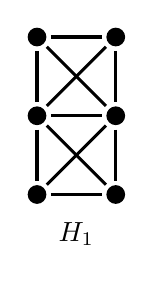
\begin{tikzpicture}[every node/.style={vertex, fill=black}, node
            distance=1cm, on grid, edge, baseline=(current bounding box.center)]
            \node (a) {};
            \node (b) [right= of a] {};
            \node (c) [below= of a] {};
            \node (d) [right= of c] {};
            \node (e) [below= of c] {};
            \node (f) [below= of d] {};
            \node (H) [label] at (0.5, -2.5) {$H_1$};
            \draw (a) to (b);
            \draw (a) to (c);
            \draw (a) to (d);
            \draw (b) to (c);
            \draw (b) to (d);
            \draw (c) to (d);
            \draw (c) to (e);
            \draw (c) to (f);
            \draw (d) to (e);
            \draw (d) to (f);
            \draw (e) to (f);

        \end{tikzpicture}
        \hfill
        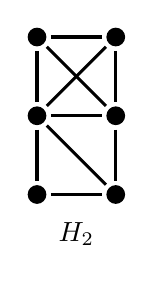
\begin{tikzpicture}[every node/.style={vertex, fill=black}, node
            distance=1cm, on grid, edge, baseline=(current bounding box.center)]
            \begin{scope}
                \node (a) {};
                \node (b) [right= of a] {};
                \node (c) [below= of a] {};
                \node (d) [right= of c] {};
                \node (e) [below= of c] {};
                \node (f) [below= of d] {};
                \node (H) [label] at (0.5, -2.5) {$H_2$};
                \draw (a) to (b);
                \draw (a) to (c);
                \draw (a) to (d);
                \draw (b) to (c);
                \draw (b) to (d);
                \draw (c) to (d);
                \draw (c) to (e);
                \draw (c) to (f);
                \draw (d) to (f);
                \draw (e) to (f);
            \end{scope}
        \end{tikzpicture}
        \hfill
        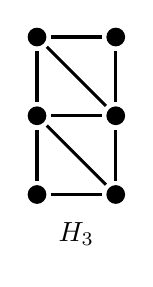
\begin{tikzpicture}[every node/.style={vertex, fill=black}, node
            distance=1cm, on grid, edge, baseline=(current bounding box.center)]

            \begin{scope}
                \node (a) {};
                \node (b) [right= of a] {};
                \node (c) [below= of a] {};
                \node (d) [right= of c] {};
                \node (e) [below= of c] {};
                \node (f) [below= of d] {};
                \node (H) [label] at (0.5, -2.5) {$H_3$};
                \draw (a) to (b);
                \draw (a) to (c);
                \draw (a) to (d);
                \draw (b) to (d);
                \draw (c) to (d);
                \draw (c) to (e);
                \draw (c) to (f);
                \draw (d) to (f);
                \draw (e) to (f);
            \end{scope}
        \end{tikzpicture}
        \hfill
        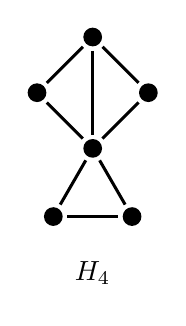
\begin{tikzpicture}[every node/.style={vertex, fill=black}, node
            distance=1cm, on grid, edge, baseline=(current bounding box.center)]
            \begin{scope}
                \node (a) {};
                \node (b) [below right= of a] {};
                \node (c) [below left= of a] {};
                \node (d) [below left= of b] {};
                \node (e) at ($(d) + (240:1)$) {};
                \node (f) at ($(d) + (300:1)$) {};
                \node (H) [label] at (0, -3) {$H_4$};
                \draw (a) to (b);
                \draw (a) to (c);
                \draw (a) to (d);
                \draw (b) to (d);
                \draw (c) to (d);
                \draw (d) to (f);
                \draw (d) to (e);
                \draw (e) to (f);
            \end{scope}
        \end{tikzpicture}
        \hfill

        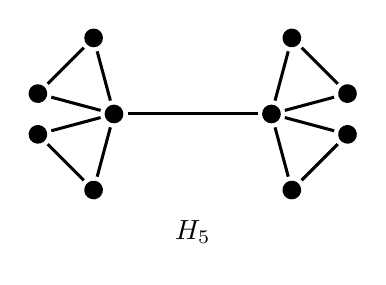
\begin{tikzpicture}[every node/.style={vertex, fill=black}, node
            distance=1cm, on grid, edge, baseline=(current bounding box.center)]
            \begin{scope}
                \node (a) at (-1,0) {};
                \node (b) [right=2 of a] {};
                \node (c) at ($(a) + (105:1)$) {};
                \node (d) [rotate around={165:(a)}] {};
                \node (e) [rotate around={-105:(a)}] {};
                \node (f) [rotate around={-165:(a)}] {};
                \node (g) [rotate around={-105:(b)}] {};
                \node (h) [rotate around={-165:(b)}] {};
                \node (i) [rotate around={105:(b)}] {};
                \node (j) [rotate around={165:(b)}] {};
                \node (H) [label] at (0, -1.5) {$H_5$};
                \draw (a) to (b);
                \draw (a) to (c);
                \draw (a) to (d);
                \draw (a) to (e);
                \draw (a) to (f);
                \draw (c) to (d);
                \draw (e) to (f);
                \draw (b) to (g);
                \draw (b) to (h);
                \draw (b) to (i);
                \draw (b) to (j);
                \draw (g) to (h);
                \draw (i) to (j);
            \end{scope}
        \end{tikzpicture}
        \hfill
        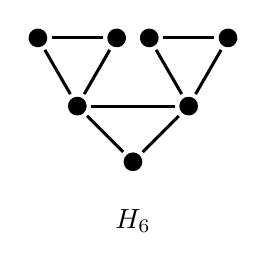
\begin{tikzpicture}[every node/.style={vertex, fill=black}, node
            distance=1cm, on grid, edge, baseline=(current bounding box.center)]
            \begin{scope}
                \node (a) {};
                \node (b) [above right= of a] {};
                \node (c) [above left= of a] {};
                \node (d) [rotate around={-105:(b)}] {};
                \node (e) [rotate around={-165:(b)}] {};
                \node (f) [rotate around={105:(c)}] {};
                \node (g) [rotate around={165:(c)}] {};
                \node (H) [label] at (0, -0.75) {$H_6$};
                \draw (a) to (b);
                \draw (a) to (c);
                \draw (b) to (c);
                \draw (b) to (d);
                \draw (b) to (e);
                \draw (d) to (e);
                \draw (c) to (f);
                \draw (c) to (g);
                \draw (f) to (g);
            \end{scope}
        \end{tikzpicture}
        \hfill
        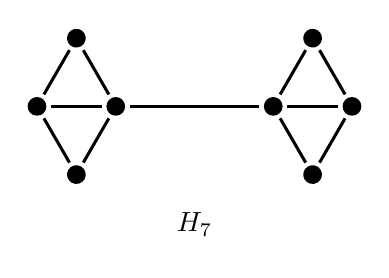
\begin{tikzpicture}[every node/.style={vertex, fill=black}, node
            distance=1cm, on grid, edge, baseline=(current bounding box.center)]
            \begin{scope}
                \node (a) at (-1,0) {};
                \node (b) [right=2 of a] {};
                \node (c) [rotate around={120:(a)}] {};
                \node (d) [rotate around={180:(a)}] {};
                \node (e) [rotate around={240:(a)}] {};
                \node (f) [rotate around={-120:(b)}] {};
                \node (g) [rotate around={-180:(b)}] {};
                \node (h) [rotate around={-240:(b)}] {};
                \node (H) [label] at (0, -1.5) {$H_7$};
                \draw (a) to (b);
                \draw (a) to (c);
                \draw (a) to (d);
                \draw (a) to (e);
                \draw (c) to (d);
                \draw (d) to (e);
                \draw (b) to (f);
                \draw (b) to (g);
                \draw (b) to (h);
                \draw (f) to (g);
                \draw (g) to (h);
            \end{scope}
        \end{tikzpicture}
        \hfill
    }
    \caption{The minimal obstructions for monopolarity in chordal
    $P_5$-free graphs.}
    \label{fig:chordal-p5-free-obstructions}
\end{figure}

\begin{proposition}
    A connected chordal $(P_5,\text{house})$-free graph with an induced $P_4$ is
    monopolar if and only if it does not contain any of the graphs depicted in
    \Cref{fig:chordal-p5-free-obstructions} as an induced subgraph.
\end{proposition}

\begin{proof}
    \leavevmode \par
    \begin{description}
        \item[$\boxed{\Rightarrow}$] \todo{Probar que cada una de las graficas de la figura no es monopolar y es
        minima}
        \item[$\boxed{\Leftarrow}$] Let $G$ be a chordal
        $(P_5,\text{house})$-free graph that does not contain any of the graphs
        depicted in \Cref{fig:chordal-p5-free-obstructions}.

        Let $P=(a,b,c,d)$ be an induced $P_4$ in $G$ and let $V=\l{a,b,c,d}$. By (i)
        and (ii) of \Cref{lem:neighborhoods-chordal}, the only possible non-empty
        sets are
        \[
            N_{b}, N_{c}, N_{ab}, N_{bc}, N_{cd}, N_{abc}, N_{bcd}, N_V 
            \text{ and } N_{\varnothing}.
        \]
        By (iii) of \Cref{lem:neighborhoods-chordal}, along with the fact that
        $G$ is $H_6$-free, we must have that each vertex in $N_{bc}$ is adjacent
        to at least one vertex in $N_{ab} \cup N_{cd}$. Nonetheless, if all
        three are non-empty, the aforementioned fact implies that $G$ would have
        a $P_5$. Thus, not all three can be non-empty, so two cases arise:

        \paragraph{Caso A} Mejora usa esto en lugar de items.

        \begin{itemize}
            \item $N_{ab} = \varnothing$ (symmetric to $N_{cd} = \varnothing$). From
            here, two new cases arise:
            \begin{itemize}
                \item $N_{cd}$ is not a clique. Let $x$ and $y$ be two
                non-adjacent vertices in $N_{cd}$. Let $K$ be the vertices of
                $N_{cd}$ that are adjacent to at least one vertex in $N_c$. We
                claim that $K$ is a clique. If not, there are $v$ and $w$ in $K$
                that are not adjacent. If a single vertex $u$ in $N_c$ is
                adjacent to both $v$ and $w$, then $\p{u,v,d,w,u}$ is a $C_4$.
                Then, there is a vertex $u$ is adjacent to just one of them, say
                $v$. Similarly, there is a vertex $u'$ in $N_c$ that is adjacent
                to just $w$. Then, notice that $\l{u,v,d,w,u'}$ induces either a
                $P_5$ or a $C_5$, depending on whether $u'$ is adjacent to $u$
                or not. Then $K$ is a clique and $N_{cd}\setminus K$ is
                anticomplete to $N_c$.
                
                Now, for each edge $vw$ in $G[N_{cd}\setminus K]$, we claim
                thatat least one of $v$ and $w$ is complete to $K$. If not,
                there are vertices $v'$ and $w'$ in $K$ such that $v'$ is not
                adjacent to $v$ and $w'$ is not adjacent to $w$. Since $v'$ is
                in $K$, there is some vertex $u$ in $N_c$ that is adjacent to
                $v'$. Since $G$ is $H_2$-free and $v$ is not adjacent to $v'$,
                it follows that $v'$ is adjacent to $w$. Similarly, $w'$ is
                adjacent to $v$. Then, $\p{v,w',v',w,v}$ is a $C_4$, a
                contradiction. Hence, vertices of $N_{cd}\setminus K$ can be
                partitioned into two sets, $S$ and $K'$, such that $S$ is stable
                and $K'$ are vertices that are complete to $K$, with the
                additional property that $S$ is maximal, that is, every vertex
                in $K'$ is adjacent to at least one vertex in $S$. We claim that
                $K'$ is a clique. If not, there are two vertices that are not
                adjacent, say $v$ and $w$. By the maximality of $S$, there are
                vertices $v'$ and $w'$ in $S$ such that $v$ is adjacent to $v'$
                and $w$ is adjacent to $w'$. If $v'\neq w'$,
                \todo{terminar este caso}
                
                Since $G$ is $H_4$-free, vertices in $N_{bc}$ must be adjacent
                to at least one of $x$ and $y$. If $w\in N_{bc}$ is adjacent to
                just one, say $x$, then $\p{b,w,x,d,y}$ is a $P_5$. Hence, $w$
                is also adjacent to $y$, but then $\p{w,x,d,y,w}$ is a $C_4$.
                Thus, $N_{bc}$ must be empty. The same argument applies to see
                that $N_{abc}$ is empty.

                By (v) of \Cref{lem:neighborhoods-chordal}, $N_{bcd}$ is
                complete to $N_{cd}$, while (iv) of the same lemma implies that
                $N_{bcd}$ is a clique.
                
                For a $w$ in $N_V$, the set $\l{a,b,c,d,w,x}$ induces either
                $H_2$ or $H_3$, depending on whether $w$ is adjacent to $x$ or
                not, respectively. Thus, $N_V = \varnothing$ (this last argument
                actually says that $N_{cd}$ not empty implies $N_V =
                \varnothing$).

                Since $G$ is $H_7$-free and $N_b$ is anticomplete to $N_{cd}$ by
                (iii) of \Cref{lem:neighborhoods-chordal}, it follows that $N_b$
                is $P_3$-free. Furthermore, since $G$ is $H_2$-free, $N_b$ is
                anticomplete to $N_{bcd}$.

                For $N_\varnothing$, by (vi) of
                \Cref{lem:neighborhoods-chordal}, each connected component of
                $G[N_\varnothing]$ is complete to at least one vertex of
                $N_{bcd}$, since this is the only non-empty set to which it can
                be adjacent. Since $G$ is $H_4$-free and $N_{bcd}$ is complete
                to $N_{cd}$, each component of $G[N_\varnothing]$ is trivial,
                that is, $N_\varnothing$ is an independent set.

                Finally, suppose $v$ and $w$ are two adjacent vertices in $N_c$.
                Since $G$ is $H_4$-free, at least one between $v$ and $w$ is
                adjacent to at least one vertex between $x$ and $y$. Say $v$ is
                adjacent to $x$. Notice $v$ is not adjacent to $y$, otherwise,
                $\p{v,x,d,y,v}$ is a $C_4$. By the same argument, $w$ cannot be
                adjacent to both $x$ and $y$, otherwise $\p{w,x,d,y,w}$ is a
                $C_4$. On the one hand, since $G$ is chordal, in particular is
                $C_5$-free, so $w$ cannot be adjacent to $y$. On the other hand,
                since $G$ is $H_2$-free, $w$ cannot be adjacent to $x$. Then,
                $\p{w,v,x,d,y}$ is a $P_5$, a contradiction. Hence, $N_c$ is an
                independent set.

                Hence, $(S\cup N_\varnothing \cup N_c,K\cup K'\cup N_{bcd}\cup
                N_b)$ is a monopolar partition of $G$.
            \end{itemize}
        \end{itemize}
    \end{description}
\end{proof}

\section{\texorpdfstring{$(P_5,\text{house})$}{(P5,house)}-free graphs with \texorpdfstring{$C_5$}{C5}}
\label{sec:c5}

\begin{proposition}
    Up to symmetry, there is only one monopolar partition of $C_5$.
\end{proposition}

\begin{proposition}
    Let $G$ be a $(P_5,\text{house})$-free graph containing an induced $C_5$. If
    $G$ is a minimal obstruction for monopolarity, then every vertex must be
    adjacent to at least one vertex of the $C_5$.
\end{proposition}

\begin{proposition}
    Let $G$ be a $(P_5,\text{house})$-free monopolar graph with an induced
    $C_5$. Let $C$ be a $C_5$ in $G$. Then:
    \begin{enumerate}[(i)]
        \item For every pair of consective vertices $x$ and $y$ in $C$,
        $N_{xy}=\varnothing$.
        \item For every vertex $x$ in $C$, $N_x = \varnothing$.
        \item For every four vertices $w$, $x$, $y$ and $z$ in $C$, $N_{wxyz}=\varnothing$.
        \item For every triple of vertices non-consecutive vertices $x$, $y$ and $z$ in $C$,
        $N_{xyz}=\varnothing$.
    \end{enumerate}
\end{proposition}

\begin{figure}[h]
    \centering
    \parbox{0.8\linewidth}{
        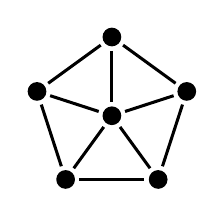
\begin{tikzpicture}[every node/.style={vertex, fill=black}, node
            distance=1cm, on grid, edge, baseline=(current bounding box.center)]
            \foreach \i in {0,...,4} \node (\i)  at ({(360/5)*\i + 90}:1){};

                \node (5) at (0,0) {};
                
                \foreach \i in {0,...,4}{
                    \draw let \n1={int(mod(\i+1,5))} in (\i) to (\n1);
                    \draw (\i) to (5);
                }
        \end{tikzpicture}
        \hfill
        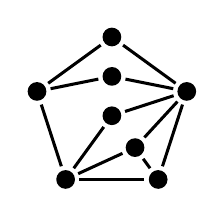
\begin{tikzpicture}[every node/.style={vertex, fill=black}, node
            distance=1cm, on grid, edge, baseline=(current bounding box.center)]
                \foreach \i in {0,...,4} \node (\i)  at ({(360/5)*\i + 90}:1){};
                    \node (5) at (0,0.5) {};
                    \node (6) at ({(360/5)*3 + 90}:0.5) {};
                    \node (7) at (0,0) {};
                    
                    \foreach \i in {0,...,4}{
                        \draw let \n1={int(mod(\i+1,5))} in (\i) to (\n1);
                    }
                    \draw (1) to (5);
                    \draw (4) to (5);
                    \draw (4) to (6);
                    \draw (2) to (6);
                    \draw (3) to (6);
                    \draw (4) to (7);
                    \draw (2) to (7);
        \end{tikzpicture}
        \hfill
        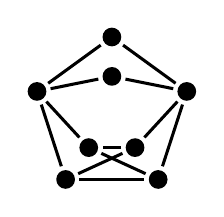
\begin{tikzpicture}[every node/.style={vertex, fill=black}, node
            distance=1cm, on grid, edge, baseline=(current bounding box.center)]
                \foreach \i in {0,...,4} \node (\i)  at ({(360/5)*\i + 90}:1){};
                    \node (5) at (0,0.5) {};
                    \node (6) at ({(360/5)*3 + 90}:0.5) {};
                    \node (7) at ({(360/5)*2 + 90}:0.5) {};
                    
                    \foreach \i in {0,...,4}{
                        \draw let \n1={int(mod(\i+1,5))} in (\i) to (\n1);
                    }
                    \draw (1) to (5);
                    \draw (4) to (5);
                    \draw (4) to (6);
                    \draw (2) to (6);
                    \draw (1) to (7);
                    \draw (3) to (7);
                    \draw (6) to (7);
        \end{tikzpicture}
        \hfill
        
        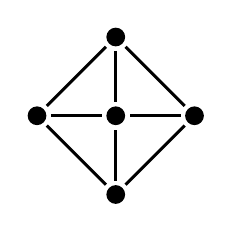
\begin{tikzpicture}[every node/.style={vertex, fill=black}, node
            distance=1cm, on grid, edge, baseline=(current bounding box.center)]
                \foreach \i in {0,...,3} \node (\i)  at ({(360/4)*\i + 90}:1){};

                    \node (4) at (0,0) {};
                    
                    \foreach \i in {0,...,3}{
                        \draw let \n1={int(mod(\i+1,4))} in (\i) to (\n1);
                        \draw (\i) to (4);
                    }
        \end{tikzpicture}
        \hfill
        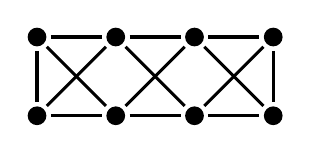
\begin{tikzpicture}[every node/.style={vertex, fill=black}, node
            distance=1cm, on grid, edge, baseline=(current bounding box.center)]
                \node (1) {};
                \node (2) [right= of 1] {};
                \node (3) [right= of 2] {};
                \node (4) [right= of 3] {};
                \node (5) [below= of 1] {};
                \node (6) [below= of 2] {};
                \node (7) [below= of 3] {};
                \node (8) [below= of 4] {};

                \draw (1) to (2);
                \draw (2) to (3);
                \draw (3) to (4);
                \draw (1) to (5);
                \draw (4) to (8);
                \draw (5) to (6);
                \draw (6) to (7);
                \draw (7) to (8);
                \draw (1) to (6);
                \draw (2) to (5);
                \draw (2) to (7);
                \draw (3) to (6);
                \draw (3) to (8);
                \draw (4) to (7);
        \end{tikzpicture}
        \hfill
        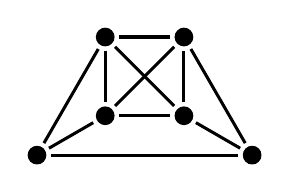
\begin{tikzpicture}[every node/.style={vertex, fill=black}, node
            distance=1cm, on grid, edge, baseline=(current bounding box.center)]
                \node (1) {};
                \node (2) [right= of 1] {};
                \node (3) [below= of 2] {};
                \node (4) [left= of 3] {};
                \node (5) at ($(4) + (-150:1)$) {};
                \node (6) at ($(3) + (-30:1)$) {};

                \draw (1) to (2);
                \draw (1) to (3);
                \draw (1) to (4);
                \draw (2) to (3);
                \draw (2) to (4);
                \draw (3) to (4);
                \draw (6) to (2);
                \draw (6) to (3);
                \draw (5) to (1);
                \draw (5) to (4);
                \draw (5) to (6);

        \end{tikzpicture}
    }
    
    \caption{The minimal obstructions for monopolarity in
    $(P_5,\text{house})$-free graphs containing an induced $C_5$.}
    \label{fig:p5-house-obstruction-with-c5}
\end{figure}

\begin{proposition}
    A $(P_5,\text{house})$-free graph $G$ with and induced $C_5$ is monopolar if
    and only if it does not contain any of the graphs depicted in
    \Cref{fig:p5-house-obstruction-with-c5} as an induced subgraph.
\end{proposition}

% TO DO: Structure of monopolar partitions given a C5
% TO DO: Lemma of minimal obstructions containing a C5
% TO DO: Algorithm for monopolarity in C5-containing graphs

\section{\texorpdfstring{$(P_5,\text{house})$}{(P5,house)}-free graphs without
\texorpdfstring{$C_5$}{C5}}
\label{sec:no-c5}

\begin{figure}[ht]
    \centering
    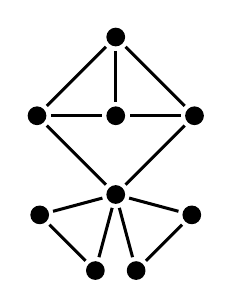
\begin{tikzpicture}[every node/.style={vertex, fill=black}, node
        distance=1cm, on grid, edge, baseline=(current bounding box.center)]
        \foreach \i in {0,...,3} \node (\i)  at ({(360/4)*\i + 90}:1){};

                \node (4) at (0,0) {};
                \node (5) at ($(2) + (195:1)$) {};
                \node (6) at ($(2) + (255:1)$) {};
                \node (7) at ($(2) + (-15:1)$) {};
                \node (8) at ($(2) + (-75:1)$) {};
                
                \foreach \i in {0,...,3}{
                    \draw let \n1={int(mod(\i+1,4))} in (\i) to (\n1);
                }
                \draw (0) to (4);
                \draw (1) to (4);
                \draw (3) to (4);
                \draw (2) to (5);
                \draw (2) to (6);
                \draw (2) to (7);
                \draw (2) to (8);
                \draw (5) to (6);
                \draw (7) to (8);
    \end{tikzpicture}
    \caption{A minimal obstruction for monopolarity in $(P_5,\text{house})$-free graphs without an induced $C_5$.}
    \label{fig:p5-house-obstruction-no-c5}
\end{figure}

\begin{proposition}
    A $(P_5,\text{house})$-free graph $G$ with no induced $C_5$ is monopolar if
    and only if it does not contain any of the previous minimal obstructions
    which are $C_5$-free and the graph depicted in
    \Cref{fig:p5-house-obstruction-no-c5} as an induced subgraph.
\end{proposition}




\backmatter

\printindex
\include{bibliografia}

\end{document}
